\pagebreak
\section*{Sample size and power (one-sample)}
\label{sampleSizeAndPower}

The Type 2 Error rate and the magnitude of the error for a point estimate are controlled by the sample size. Real differences from the null value, even large ones, may be difficult to detect with small samples. If we take a very large sample, we might find a statistically significant difference but the magnitude might be so small that it is of no practical value. In this section we describe techniques for selecting an appropriate sample size based on these considerations for a single mean.

\subsection{Finding a sample size for a certain margin of error}
\label{findingASampleSizeForACertainME}

\index{margin of error|(}

Many companies are concerned about rising healthcare costs. A company may estimate certain health characteristics of its employees, such as blood pressure, to project its future cost obligations. However, it might be too expensive to measure the blood pressure of every employee at a large company, and the company may choose to take a sample instead.

\begin{example}{Blood pressure oscillates with the beating of the heart, and the systolic pressure is defined as the peak pressure when a person is at rest. The average systolic blood pressure for people in the U.S. is about 130 mmHg with a standard deviation of about 25 mmHg. How large of a sample is necessary to estimate the average systolic blood pressure with a margin of error of 4 mmHg using a 95\% confidence level?}
\label{sampleSizeComputationForSystolicBloodPressure}
First, we frame the problem carefully. Recall that the margin of error is the part we add and subtract from the point estimate when computing a confidence interval. The margin of error for a 95\% confidence interval estimating a mean can be written as
\begin{align*}
ME_{95\%} = 1.96\times SE = 1.96\times\frac{\sigma_{employee}}{\sqrt{n}}
\end{align*}
The challenge in this case is to find the sample size $n$ so that this margin of error is less than or equal to 4, which we write as an inequality:
\begin{align*}
1.96\times \frac{\sigma_{employee}}{\sqrt{n}} \leq 4
\end{align*}
In the above equation we wish to solve for the appropriate value of $n$, but we need a value for $\sigma_{employee}$ before we can proceed. However, we haven't yet collected any data, so we have no direct estimate! Instead, we use the best estimate available to~us: the approximate standard deviation for the U.S. population, 25. To proceed and solve for $n$, we substitute 25 for $\sigma_{employee}$:
\begin{align*}
1.96\times \frac{\sigma_{employee}}{\sqrt{n}} \approx 1.96\times\frac{25}{\sqrt{n}}
	&\leq 4 \\
1.96\times\frac{25}{4} &\leq \sqrt{n} \\
\left(1.96\times\frac{25}{4}\right)^2 &\leq n \\
150.06 &\leq n
\end{align*}
This suggests we should choose a sample size of at least 151 employees. We round up because the sample size must be \emph{greater than or equal to 150.06}.
\end{example}

A potentially controversial part of Example~\ref{sampleSizeComputationForSystolicBloodPressure} is the use of the U.S. standard deviation for the employee standard deviation. Usually the standard deviation is not known. In~such cases, it is reasonable to review scientific literature or use market research to make an educated guess about the standard deviation.

\begin{termBox}{\tBoxTitle{Identify a sample size for a particular margin of error}
To estimate the necessary sample size for a maximum margin of error $m$, we set up an equation to represent this relationship:
\begin{align*}
m \geq ME = z^{\star}\frac{\sigma}{\sqrt{n}}
\end{align*}
where $z^{\star}$ is chosen to correspond to the desired confidence level, and $\sigma$ is the standard deviation associated with the population. Solve for the sample size,~$n$:
\begin{align*}
n \geq \left(z^{\star} \frac{\sigma}{m}\right)^2
\end{align*}}
\end{termBox}

Sample size computations are helpful in planning data collection, and they require careful forethought. Next we consider another topic important in planning data collection and setting a sample size: the Type 2 Error rate.

\index{margin of error|)}


\subsection{Power and the Type 2 Error rate}

Consider the following two hypotheses:
\begin{itemize}
\setlength{\itemsep}{0.5mm}
\item[$H_0$:] The average blood pressure of employees is the same as the national average, $\mu = 130$.
\item[$H_A$:] The average blood pressure of employees is different than the national average, $\mu \neq 130$.
\end{itemize}
Suppose the alternative hypothesis is actually true. Then we might like to know, what is the chance we make a Type 2 Error? That is, what is the chance we will fail to reject the null hypothesis even though we should reject it? The answer is not obvious! If the average blood pressure of the employees is 132 (just 2 mmHg from the null value), it might be very difficult to detect the difference unless we use a large sample size. On the other hand, it would be easier to detect a difference if the real average of employees was 140.

\begin{example}{Suppose the actual employee average is 132 and we take a sample of 100 individuals. Then the true sampling distribution of $\bar{x}$ is approximately $N(132, 2.5)$ (since $SE \approx \frac{25}{\sqrt{100}} = 2.5$). What is the probability of successfully rejecting the null hypothesis?}
\label{computePowerIfMuIs132AndMu0Is130}
This problem can be divided into two normal probability questions. First, we identify what values of $\bar{x}$ would represent sufficiently strong evidence to reject $H_0$. Second, we use the hypothetical sampling distribution with center $\mu=132$ to find the probability of observing sample means in the areas we found in the first step.

\textbf{Step 1.} The null distribution could be represented by $N(130, 2.5)$, the same standard deviation as the true distribution but with the null value as its center. Then we can find the two tail areas by identifying the $Z$ score corresponding to the 2.5\% tails ($\pm 1.96$), and solving for $x$ in the Z-score equation:
\begin{align*}
-1.96 = Z_1 &= \frac{x_1 - 130}{2.5}
	&+1.96 = Z_2 &= \frac{x_2 - 130}{2.5} \\
x_1 &= 125.1
	&x_2 &= 134.9
\end{align*}
(An equally valid approach is to recognize that $x_1$ is $1.96\times SE$ below the mean and $x_2$ is $1.96\times SE$ above the mean to compute the values.) Figure~\ref{power132And141} shows the null distribution on the left with these two dotted cutoffs.

\textbf{Step 2.} Next, we compute the probability of rejecting $H_0$ if $\bar{x}$ actually came from $N(132, 2.5)$ \emph{and} is in the direction of the truth (above 130~mmHg). This is the same as finding the shaded tail for the second distribution in Figure~\ref{power132And141}. We use the Z-score method:
\begin{align*}
Z_{right} &= \frac{134.9 - 132}{2.5} = 1.16
	&&area_{right} =0.123
\end{align*}
The probability of rejecting the null mean, if the true mean is 132, is 0.123.
\end{example}

\begin{figure}[ht]
\centering
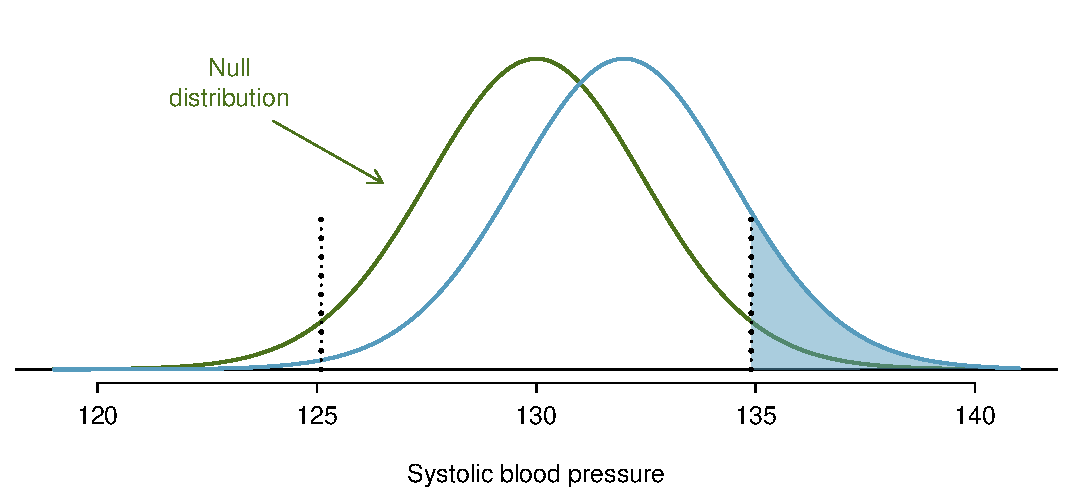
\includegraphics[width=\textwidth]{power/OneSampleIntroduction/power132And141/power132And141}
\caption{The sampling distribution of $\bar{x}$ under two scenarios. Left: $N(130, 2.5)$. Right: $N(132, 2.5)$, and the shaded area in this distribution represents the power of the test.}
\label{power132And141}
\end{figure}

The probability of rejecting the null hypothesis is called the \term{power}. The power varies depending on what we suppose the truth might be. In Example~\ref{computePowerIfMuIs132AndMu0Is130}, the difference between the null value and the supposed true mean was relatively small, so the power was also small: only 0.123. However, when the truth is far from the null value, where we use the standard error as a measure of what is far, the power tends to increase.

\begin{exercise}
Suppose the true sampling distribution of $\bar{x}$ is centered at 140. That is, $\bar{x}$ comes from $N(140, 2.5)$. What would the power be under this scenario? It may be helpful to draw $N(140, 2.5)$ and shade the area representing power on Figure~\ref{power132And141}; use the same cutoff values identified in Example~\ref{computePowerIfMuIs132AndMu0Is130}.\footnote{Draw the distribution $N(140, 2.5)$, then find the area above 134.9: about 0.979. If the true mean is 140, the power is about 0.979.}
\end{exercise}

\begin{exercise}
If the power of a test is 0.979 for a particular mean, what is the Type~2 Error rate for this mean?\footnote{The Type 2 Error rate represents the probability of failing to reject the null hypothesis. Since the power is the probability we do reject, the Type 2 Error rate will be $1-0.979 = 0.021$.}
\end{exercise}

\begin{exercise}
Provide an intuitive explanation for why we are more likely to reject $H_0$ when the true mean is further from the null value.\footnote{Answers may vary a little. When the truth is far from the null value, the point estimate also tends to be far from the null value, making it easier to detect the difference and reject $H_0$.}
\end{exercise}

\subsection{Statistical significance versus practical significance}

When the sample size becomes larger, point estimates become more precise and any real differences in the mean and null value become easier to detect and recognize. Even a very small difference would likely be detected if we took a large enough sample. Sometimes researchers will take such large samples that even the slightest difference is detected. While we still say that difference is \term{statistically significant}, it might not be \term{practically significant}.

Statistically significant differences are sometimes so minor that they are not practically relevant. This is especially important to research: if we conduct a study, we want to focus on finding a meaningful result. We don't want to spend lots of money finding results that hold no practical value.

The role of a statistician in conducting a study often includes planning the size of the study. The statistician might first consult experts or scientific literature to learn what would be the smallest meaningful difference from the null value. She also would obtain some reasonable estimate for the standard deviation. With these important pieces of information, she would choose a sufficiently large sample size so that the power for the meaningful difference is perhaps 80\% or 90\%. While larger sample sizes may still be used, she might advise against using them in some cases, such as when collecting more data than is truly necessary is unethical (e.g. a clinical trial) or where collecting the data is relatively costly.
